\documentclass{cmspaper}
\def\RCS$#1: #2 ${\expandafter\def\csname RCS#1\endcsname{#2}}
\RCS$Revision: 1.5 $
\RCS$Date: 2004/06/24 20:39:24 $

\begin{document}
\begin{titlepage}
  \whitepaper
  \date{Revision \RCSRevision, \RCSDate}
  \title{CMS Data Handling: Routing System}

  \begin{Authlist}
    Tim~Barrass, Simon~Metson\Instfoot{bristol}{University of Bristol, Bristol, UK}
    Lassi~A.~Tuura\Instfoot{neu}{Northeastern University, Boston, USA}
  \end{Authlist}

  \begin{abstract}
This white paper describes the components and algorithms used by the system we use to route files to their destinations.  Our algorithm of choiceis the Routing Internet Protocol (RFC 2453) adapted for our purposes.  This document is intended to evolve as we extend the implementation to handle more complex user requirements.
  \end{abstract} 

  \note{DRAFT version}
\end{titlepage}

\setcounter{page}{2}

\section{Overview}
Here we describe the overall structure of the data distribution management system for CMS. The system is based on a not-fully-interconnected network of nodes, where network links between nodes represent an "advertising" relationship between the nodes: agents at each node will determine whether their neighbours are or should be interested in a file, and advertise it to them when available.

Routing is handled with an implementation of the Routing Internet Protocol (RFC2453), one of the simplest (and most widely used) distance vector based internet routing protocols. Our algorithm has certain modifications- principally we have chosen not to have nodes communicate with each other to determine current route information- instead, updates are made asynchronously in a central database.

The RIP describes a mechanism by which distributed routers can maintain a local table of routes to all other destinations in the system. Local routing tables are updated by passing messages between neighbouring routers.

In our system there are no distributed routing tables: instead there is a single global routing table. Distributed routing tables are effectively modelled in the central routing table, however, as each route stored is associated with the source node (the global table is effectively partitioned on the source node into separate "local" routing tables).

Population and maintenance of these "local" routing tables is undertaken by a routing agent present at each node.

\subsection{Global database tables}
The routing system is reliant on two tables in the TMDB (described in a separate white paper), although some uses of the routing system also query and update other tables (fig. \ref{fig:schema}). This white paper should be taken with the TMDB schema paper to describe the whole system.

\begin{figure}[htb]
\centering
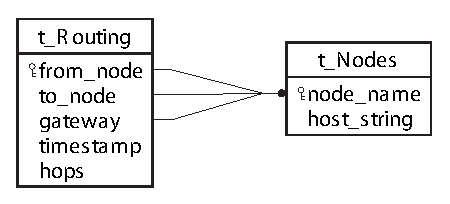
\includegraphics{v2_routing.eps}
\caption{TMDB entities and relations used in routing.}
\label{fig:schema}
\end{figure}

\section{Deployment and removal of nodes}
Deployment and removal of nodes will be quite straightforward: however, there are some situations that will require more maintenance than others, so some subtlety is required. Not all possible deployment and removal scenarios are considered here; the descriptions below should be seen as guidelines for dealing with other scenarios.

[TODO: we should build this up as more experience is gained]

\subsection{Deployment}
There are two scenarios for deployment of nodes: either the node will connect to a single other node, or will form a new link between two or more existing nodes (considered a new link) or an existing link between two nodes will be broken and a new node inserted (considered a split-link).

In general at deployment, initial entries must be made in the node register and routing tables to register nodes with each other- e.g. if A and B are deployed at time t0 then the entries

\begin{tabular}{lllll}
from\_node	& to\_node	& gateway	& hops	& timestamp	
\\ \hline A	& B	& B	& 1	& t0
\\ B	& A	& A	& 1	& t0
\end{tabular}

must be made in the routing table. Deployment of a "new link" node is this simple- note if B were to form a new route between nodes A and C then entries describing the link between B and C would also need to be made.

If a new node is to be inserted between two existing, linked nodes then the existing link must first be broken. New links can then be formed as required, as described above. Finally, outstanding transfers between the two original nodes need to be redirected. This can be achieved using the following: assume that A and C are linked, but a node B is to be inserted between them at time t1

\subsubsection{\textbf{\texttt{register node}}}

{\small\begin{verbatim}
insert into t_Nodes
  values ('B','b.cern.ch');
\end{verbatim}}

\subsubsection{\textbf{\texttt{destory existing link}}}

{\small\begin{verbatim}
delete from t_Routing
  where from_node = 'A'
    and to_node = 'C';
delete from t_Routing
  where from_node = 'C'
    and to_node = 'A';
\end{verbatim}}

\subsubsection{\textbf{\texttt{form new links}}}

{\small\begin{verbatim}
insert into t_Routing
  values ('A','B','B',t1,1);
insert into t_Routing
  values ('B','A','A',t1,1);
insert into t_Routing
  values ('C','B','B',t1,1);
insert into t_Routing
  values ('B','C','C',t1,1);
\end{verbatim}}

\subsubsection{\textbf{\texttt{redirect transfer adverts}}}

{\small\begin{verbatim}
update t_Routing
  set gateway = 'B'
  where is_for_node = 'C'
    and is_at_node = 'A'
    and state = 1;
\end{verbatim}}

\subsection{Removal}
If a node is on a spur- that is, it only connects to a single node- then removal is straightforward. If the node is connected to multiple other nodes then removal is more complex.

RIP handles removal by triggered updates: when a router is removed from the system a message is sent to other nodes to inform them; this message is propagated through the system. 

To some extent it is easier for us to remove a node from the system as all our routing information is in one place. However, our task is complicated by our need to maintain bookkeeping information on replicas in the system. Specifically, files will be advertised as available for transfer on the node to be removed. If the node is removed without dealing with these advertisements then a chain of distribution will be broken. So the full process for removing a node is

\subsubsection{\textbf{\texttt{delete from file allocation table}}}
{\small\begin{verbatim}
delete from t_File_allocation_config
  where to_node = 'Z'
    or gateway = 'Z'
    or from_node = 'Z';
\end{verbatim}}

\subsubsection{\textbf{\texttt{delete from routing table}}}

{\small\begin{verbatim}
delete from t_Routing
  where to_node = 'Z'
    or gateway = 'Z'
    or from_node = 'Z';
\end{verbatim}}

Remember which nodes were neighbours!

\subsubsection{\textbf{\texttt{form new links if necessary}}}
If the removed node connected two other nodes, and a link is still required between these nodes, then a new link must be formed. If, for example, A and C were connected through Z, then a new lnik between A and C would be forged

{\small\begin{verbatim}
insert into t_Routing
  values ('A','C','C',t1,1);
insert into t_Routing
  values ('C','A','A',t1,1);
\end{verbatim}}

\subsubsection{\textbf{\texttt{redirect replica adverts}}}
This is somewhat complex, as it involves determining where files should be sent next. Adverts for replicas that are directed toward the removed node and that are on neighbouring nodes can be ignored at this stage. 

If the route for a file extends further than the removed node then an alternate route to the destination must be found. If we wait until the global routing table has adjusted to the removal of the node then we can treat the re-advertisement as the transfer agents do- assuming that the file is available at node A, which used to neighbour Z, and is directed toward C, then the gateway is given by

{\small\begin{verbatim}
select gateway from t_Routing
  where from_node = 'A'
    and to_node = 'C';
\end{verbatim}}

(Imagine this returns B as the new gateway). An alternative advertisement then needs to be made

{\small\begin{verbatim}
insert into t_File_state
  values (guid1, 'B', 1, 'A');
\end{verbatim}}

All adverts pertaining to the removed node can then be deleted

{\small\begin{verbatim}
delete from t_File_state
  where is_for_node = 'Z';
delete from t_File_state
  where is_at_node = 'Z'
  and state = 1;
\end{verbatim}}

(Note that this will lead entries for replicas that did pass through Z hanging around: but as these transfers have already occurred this is not a problem, as long as noone relies on the replica still being there).

\subsubsection{\textbf{\texttt{discard node}}}

{\small\begin{verbatim}
delete from t_Nodes
  were name = 'Z';
\end{verbatim}}

Note that a lot of this can be handled by a global garbage collection agent.

\section{Building the routing table: registration and route sharing}
At any given node the routing agent periodically executes a variation of the RIP algorithm. There are subtle differences between our algorithm and RIP: at some stages, where RIP routers actively send their neighbours their routing information, our nodes query their neighbours "local" routing tables for routing information.

In both algorithms disappearing routes are handled by timing out direct (or node to neighbour) routes that are not refreshed within a certain time limit. The distance metric- hops- associated with routes that time out are set to some number larger than the expected maximum number of hops in the network.

\subsection{Routing algorithm}
The algorithm proceeds as follows. As with original RIP routers, our nodes "send" contact their neighbours to let them know they are still available- to avoid getting timed out. Our nodes do this by updating their single-hop entry in their neighbours tables. If the current time is t0, then a node named A would refresh its links with neighbours using

\subsubsection{\textbf{\texttt{refresh links with neighbours}}}

{\small\begin{verbatim}
update t_Routing
  set timestamp = t0
  where to_node = 'A'
    and gateway = 'A';
\end{verbatim}}

\subsubsection{\textbf{\texttt{query neighbour's routes}}}
RIP and our algorithm then have a phase in which routing information is shared between neighbours. RIP routers do this by sending their routing table to their neighbours. Our routing agents do this by querying their neighbours routing tables for information

{\small\begin{verbatim}
select from_node,to_node,timestamp,hops+1 from t_Routing
  where from_node in 
    (select from_node from t_Routing where to_node = 'A' and gateway = 'A')
    and not to_node = 'A'
  minus
  select gateway,to_node,timestamp,hops from t_Routing
  where from_node = 'A';
\end{verbatim}}

Certain provisos are implemented to speed the propagation of information- especially about timed-out routes- through the network. In principle, if a node A determines that a route to node C from a neighbouring node B comes directly back through A then it can do one of two things. It can ignore the route (termed "split horizon")- safe, as there is clearly a more direct route from A to C that A will know about. Alternatively it can retain the route but set the number of hops effectively to infinity (termed "split horizon with poisoned reverse").

Our algorithm implements split horizon with poisoned reverse, as is recommended in the router requirements RFC. It is applied to the new routes as they are returned from the SQL above.

Both RIP and our algorithm then compare the new routes they have found with their existing routes, and build a new routing table by merging the two.

\subsubsection{\textbf{\texttt{establish existing routes}}}
To establish the node's existing routes- for node A

{\small\begin{verbatim}
  select gateway,to_node,timestamp,hops from t_Routing
    where from_node = 'A';
\end{verbatim}}

The new routes are then compared with existing routes. If for a given new route the gateway and destination match, the new number of hops is taken to be accurate whether it is higher or lower than the existing hops estimate.

If for a gven new route the gateway and destination do not match, then the route with the smallest number of hops is chosen for entry into the table.

The node's routing table is then rebuilt by updating existing entries, or inserting new entries for newly found routes.

If failover is not required, then the routing algorithm stops here.
However, if failover is required, then the algorithm needs to be
modified to handle nodes that disappear.  Disappearing nodes can be
handled by effectively setting the number of hops to that node to
infinity during an expiry phase.

\subsubsection{\textbf{\texttt{maintaining the routing table: failover}}}
During this phase the agent manager examines links with each of its
neighbours (e.g. links in it's own from-partition of the table for
which to == gateway) in the routing table.  If an entry has not been
refreshed within some critical period, the number of hops is
effectively set to infinity (the RIP algorithm suggest 16, assuming
that the protocols are useful only for networks where the longest
direct routes are less than 15 hops).

The information that a link is down is then gradually propagated
throughout the table as nodes ``ask'' their neighbours (or examine
their from-partitions) for their current estimate of hops for each
route.  When the node comes back up and re-registers, it will
automatically set the number of hops to 1.

\end{document}
